%!TEX root = draft.tex
%\newcommand{\seqPQ}{\mathsf{SeqPQ}}

\section{Distributed Linearizability}
\label{sec:distributed-lin}

In this section, we propose a framework to specify the expected outcome in a linearizable approach, without referring to implementation details.



\subsection{Histories}
\label{subsec:histories} 
 

%We define our specification on histories, which are abstract version of detailed executions and does not contain implementation details such as message delivery. Histories are used to capture the notion of client-observable effects (operations), as well as their order in each replica, and their visibility relation.

%Let us introduce the notion of operations. 
A operation label $m(a) \Rightarrow b$ with $m \in \mathbb{M}$ and $a,b \in \mathbb{D}$ is the user-observable behavior of an operation, which indicates that this operation calls method $m$ with argument $a$ and its return value is $b$. $\mathbb{OID}$ is a infinite set of operation identifiers. An operation is defined to be a tuple $(\ell,i,x)$, where $\ell$ is a operation label, $i \in \mathbb{OID}$ is a unique operation identifier, and $x \in \mathbb{OBJ}$ is the objects of this operation. Let $\mathbb{OP}$ be the set of operations. For operation label $m(a) \Rightarrow b$, when the argument (resp., return value) is not used, we write $m()\Rightarrow b$ (resp., $m(a)$) instead for short.

With the notion of operations, we can now define histories.

\begin{definition}[histories]
\label{definition:histories}
A history is a tuple of the form $(\mathit{Op},\mathit{ro},\mathit{vis})$ .Here $\mathit{Op} \subseteq \mathbb{OP}$ is a set of operations; $\mathit{ro} \subseteq \mathit{Op} \times \mathit{Op}$ is the replica order, which is a union of transitive, irreflexive and total orders over $\mathit{Op}$; $\mathit{vis} \subseteq \mathit{Op} \times \mathit{Op}$ is the visibility order, which is acyclic and relates operations of same object. We require that $\mathit{ro} \subseteq \mathit{vis}$.
\end{definition}

$(o_1,o_2) \in \mathit{ro}$ represents that $o_1$ and $o_2$ are of same replica and the time point of $o_1$ is before that of $o_2$. $(o_1,o_2) \in \mathit{vis}$ means that $o_2$ is aware of $o_1$. %In detailed execution, this means that some message carrying the effect of $o_1$ has already been delivered into replica of $o_2$. In state-based CRDT implementation, this message contains some state aware of $o_1$, while in operation-based CRDT implementation, this message is the message of $o_1$. Based on this intuition, when 
We quire that for $(o_1,o_2) \in \mathit{vis}$, $o_1$ is of a update method, since only update methods have side-effect.

\subsection{Sequential Specification}
\label{subsec:sequential specification}

%A sequential specification intends to propose a linearizable explanation for distributed objects.

A specification alphabet is a tuple $(\ell,\mathit{id},S)$, where $\ell$ is a operation label, $\mathit{id}$ is an identifier of this specification alphabet, and $S$ is a set of identifiers. Let $\mathbb{A}$ be the set of specification alphabets. A sequential specification of CRDT is defined as a set of sequences over specification alphabets $\mathbb{A}$.

%\gp{We should add the specifications (even non-deterministic here.)}
\begin{definition}[Sequential Specification]
\label{definition:sequential specification}
A sequential specification is a set of strings over specification alphabet $\mathbb{A}$.
\end{definition}

The sequential specification is defined by transition rules of the form $\mathit{cond}_1$ $(m(a) \Rightarrow b,\mathit{id},S)$ $\mathit{cond}_2$, where $\mathit{cond}_1$ is a pre-condition and $\mathit{cond}_2$ is a post condition. When $\mathit{id}$ is not used in $\mathit{cond}_1$ and $\mathit{cond}_2$, we can skip it. When $S=\emptyset$, we can skip it. We write $s {\xrightarrow{(m(a) \Rightarrow b,\mathit{id},S)}} s'$, if there exists a transition rule $\mathit{cond}_1$ $(m(a) \Rightarrow b,\mathit{id},S)$ $\mathit{cond}_2$, such that $s$ satisfies $\mathit{cond}_1$ and $s'$ satisfies $\mathit{cond}_2$. A sequence $(\ell_1,\mathit{id}_1,S_1) \cdot \ldots \cdot (\ell_k,\mathit{id}_k,S_k)$ is in sequential specification, if there exists state $s_k$, such that $s_0 {\xrightarrow{(\ell_1,\mathit{id}_1,S_1)}} \ldots {\xrightarrow{(\ell_k,\mathit{id}_k,S_k)}} s_k$, and $s_0$ is the initial state. Here we also require that each $\mathit{id}$ is unique in $(\ell_1,\mathit{id}_1,S_1) \cdot \ldots \cdot (\ell_k,\mathit{id}_k,S_k)$. 



%For objects of simple types, a sequential specification is a set of operation sequences. Normally, the sequential specification is defined by the pre-condition and post-conditions. For example, the following is the sequential specification for distributed counter, and is given as a set of transition rules between states. Each state contains a integer value. Transition rule $\{ \mathit{state} = i \}$ $(\mathit{inc},\_,\_)$ $\{ \mathit{state} = i+1 \}$ indicates that $\mathit{inc}$ will increase the state by $1$. Here we use $\_$ to indicate an element whose value has no influence. Since this rule does not use operation identifier and object, it is safe to write $\{ \mathit{state} = i \}$ $\mathit{inc}$ $\{ \mathit{state} = i+1 \}$ instead. Similarly for $\mathit{dec}$ and $\mathit{read}$ operations. We write $s {\xrightarrow{o}} s'$ to indicate one step of $o$ transition between states $s$ and $s'$ that satisfies some transition rule.

%A sequence $(\ell_1,i_1,x) \cdot \ldots \cdot (\ell_k,i_k,x)$ is in sequential specification $\mathit{counter}_s$, if there exists state $s_k$, such that $s_0 {\xrightarrow{(\ell_1,i_1,x)}} \ldots {\xrightarrow{(\ell_k,i_k,x)}} s_k$, and $s_0$ is the initial state. For example, it is easy to see that $(\mathit{inc},\mathit{id}_1,x) \cdot (\mathit{inc},\mathit{id}_2,x) \cdot (\mathit{dec},\mathit{id}_3,x) \cdot (\mathit{read} \Rightarrow 1,\mathit{id}_4,x) \in \mathit{counter}_s$. Note that operations of one sequence of $\mathit{counter}_s$ must be of a same object. We also implicitly assume that each operation has a unique operation identifier.


\begin{example}[sequential specification of counter]
\label{definition:sequential specification of counter}
The sequential specification $\mathit{counter}_s$ of counter is given as follows: Let $\mathit{state}$ be a integer with initial value $0$.

\begin{itemize}
\setlength{\itemsep}{0.5pt}
\item[-] $\{ \mathit{state} = k \}$ $\mathit{inc}$ $\{ \mathit{state} = k+1 \}$.
\item[-] $\{ \mathit{state} = k \}$ $\mathit{dec}$ $\{ \mathit{state} = k-1 \}$.
\item[-] $\{ \mathit{state} = k \}$ $(\mathit{read}() \Rightarrow i)$ $\{ \mathit{state} = k \}$.
\end{itemize}
\end{example}

%However, for objects of some types which are designed only for distributed system, such as multi-value register and OR-set, sequential specification in above style seems insufficient (we explain this in the next subsection). To solve this problem, in the transition rules of sequential specification, for some operations, we give them a additional argument which is a set of operation identifiers. Such additional argument essentially represents the operations visible to this operation. We use the sequential specification of multi-value register as example to explain this, which is shown below.

%Each state contains a set of tuples $(a,\mathit{id},f)$, where $a$ is item, $\mathit{id}$ is the operation identifier of the operation that put this tuple, and $f$ indicates whether this item is logically removed or not. Given a state $S$, a $(write(a),\mathit{id},x)$ operation with argument $S_1$, the resulting state is obtained by marking all items in $S$ with $S_1$ identifiers into $\mathit{false}$, and then insert $(a,id,\mathit{true})$ into $S$. A $\mathit{read}$ operation returns value with flag $\mathit{true}$ in state.


\begin{example}[sequential specification of multi-value register]
\label{definition:sequential specification of multi-value register}
The sequential specification $\mathit{MVReg}_s$ of multi-value register is given as follows: Let $\mathit{state}$ be a set and each its element $(a,\mathit{id},f)$ is a tuple of a data $a$, a operation identifier $\mathit{id} \in \mathbb{O}$, and a flag $f \in \{ \mathit{true},\mathit{false} \}$.
\begin{itemize}
\setlength{\itemsep}{0.5pt}
\item[-] $\{ \mathit{state} = S \}$ $(write(a),\mathit{id},S_1)$ $\{ \mathit{state} = S[(b,\mathit{id}_1) \in S_2 : \mathit{false}]
\cup
\{ (a,id,\mathit{true}) \}
\}$. Here $S_2 = \{ (b,\mathit{id}_1) \vert (b,\mathit{id}_1,\mathit{true}) \in S \wedge id \in S_1 \}$.
\item[-] $\{ \mathit{state} = S \wedge S_1 = \{ a \vert (a,\_,\mathit{true}) \in S \} \}$ $read() \Rightarrow S_1$ $\{ \mathit{state} = S \}$.
\end{itemize}
\end{example}


%The methods that needs additional arguments, such as $\mathit{write}$ method of multi-value register and $\mathit{rem}$ method of OR-set, is called special methods of that specification. Given a sequential specification  A sequential specification is $\mathit{deterministic}$, if in each of its rules, from each state with each operation, there is at most one resulting state. Otherwise, it is a $\mathit{nondeterministic}$ specification. In the following we will introduce several types and their sequential specifications. $\mathit{list}_s^{\mathit{ab}}$, a version of list specification, is nondeterministic, while all other sequential specifications are deterministic.


\begin{example}[set and its sequential specification]
\label{definition:sequential specification of set}
A set has three methods: $\mathit{add}(a)$ inserts item $a$ into set; $\mathit{rem}(a)$ removes $a$ from set; and $\mathit{read}$ returns the set content. It implicitly assumes that each item being put into the set only once. The sequential specification $\mathit{set}_s$ of set is given as follows:  Let $\mathit{state}$ be a set and each its element $(a,f)$ is a tuple of a data $a$ and a flag $f \in \{ \mathit{true},\mathit{false} \}$.

\begin{itemize}
\setlength{\itemsep}{0.5pt}
\item[-] $\{ \mathit{state} = S \wedge a \notin S \}$ $\mathit{add}(a)$ $\{ \mathit{state} = S \cup \{ (a,\mathit{true}) \} \}$.
\item[-] $\{ \mathit{state} = S \wedge (a,\_) \in S \}$ $\mathit{rem}(a)$ $\{ \mathit{state} = S[a:\mathit{false}] \}$.
\item[-] $\{ \mathit{state} = S \wedge S_1 = \{a \vert (a,\mathit{true}) \in S \} \}$ $(\mathit{read}() \Rightarrow S_1)$ $\{ \mathit{state} = S \}$.
\end{itemize}
\end{example}



\begin{example}[OR-set and its sequential specification]
\label{definition:sequential specification of or-set}
OR-set is essential a multi-set: $\mathit{add}(a)$ inserts an item $a$ into multi-set; $\mathit{rem}(a)$ cancels only items $a$ that are inserted by $\mathit{add}(a)$ operations visible to this remove operation; $\mathit{read}$ returns the set of items in multi-set. A value can be inserted multiple times.

The sequential specification $\mathit{OR}$-$\mathit{set}_s$ of OR-set is given as follows: Let $\mathit{state}$ be a set and each its element $(a,\mathit{id},f)$ is a tuple of a data $a$, a operation identifier $\mathit{id} \in \mathbb{O}$, and a flag $f \in \{ \mathit{true},\mathit{false} \}$. %In $((rem(a),\mathit{id}'),S_1)$, $S_1$ represents the operations visible to this remove operation.
\begin{itemize}
\setlength{\itemsep}{0.5pt}
\item[-] $\{ \mathit{state} = S  \wedge (\_,\mathit{id},\_) \notin S \}$ $(\mathit{add}(a),\mathit{id})$ $\{ \mathit{state} = S \cup \{ (a,\mathit{id},\mathit{true}) \} \}$.
\item[-] $\{ \mathit{state} = S \wedge S_1 = \{ a \vert (a,\_,\mathit{true}) \in S \} \}$ $(\mathit{read}() \Rightarrow S_1)$ $\{ \mathit{state} = S \}$.
\item[-] $\{ \mathit{state} = S \}$ $(rem(a),S_1)$ $\{ \mathit{state} = S[(b,\mathit{id}_1) \in S_2 : \mathit{false}] \}$. Here $S_2 = \{ (b,\mathit{id}_1) \vert (b,\mathit{id}_1,\mathit{true}) \in S \wedge id \in S_1 \}$.
\end{itemize}
\end{example}


\begin{example}[register and its sequential specification]
\label{definition:sequential specification of register}
A register has two methods: $\mathit{write}(a)$ writes $a$ into register; $\mathit{read}$ returns the value of register. The sequential specification $\mathit{reg}_s$ of register is given as follows: Let $\mathit{state} \in \mathbb{D}$ be a value.
\begin{itemize}
\setlength{\itemsep}{0.5pt}
\item[-] $\{ \mathit{state} = a  \}$ $\mathit{write}(b)$ $\{ \mathit{state} = b \}$.
\item[-] $\{ \mathit{state} = a \}$ $(\mathit{read}() \Rightarrow a)$ $\{ \mathit{state} = a \}$.
\end{itemize}
\end{example}




\begin{example}[List with add-after interface]
\label{definition:sequential specification of list with add-after interface}
Assume each item of the list is unique. A list has three methods: $\mathit{add}(b,a)$ inserts item $b$ into the list at the position immediately after that of item $a$; $\mathit{rem}(a)$ removes item $a$ from the list; and $\mathit{read}$ returns the list content. We assume that the initial value of list is $(\circ,\mathit{true})$ and this node can not be removed. We use the word ``add-after'' to emphasize the method $\mathit{add}(b,a)$, which is different from the other list interface that uses method $\mathit{add}(b,a,c)$.

The sequential specification $\mathit{list}_s^{\mathit{af}}$ of list is given as follows: Let $\mathit{state}$ be a sequence, where each item is a tuple $(a,f)$ with data $a$ and flag $f \in \{ \mathit{true},\mathit{false} \}$. Here $\mathit{af}$ represents add-after, and we use $l \uparrow_{S}$ to represent the projection of sequence $l$ into set $S$. When the context is clear, in $\mathit{read}$ operation, we will omit $\circ$.
\begin{itemize}
\setlength{\itemsep}{0.5pt}
\item[-] $\{ \mathit{state} = (a_1,f_1) \cdot \ldots \cdot (a_n,f_n) \wedge l \leq n \wedge b \notin \{ a_1, \ldots, a_n \} \}$ $add(b,a_l)$ $\{ \mathit{state} = (a_1,f_1) \cdot \ldots \cdot (a_l,f_l) \cdot (b,\mathit{true}) \cdot (a_{l+1},f_{l+1}) \cdot \ldots \cdot (a_n,f_n) \}$.
\item[-] $\{ \mathit{state} = (a_1,f_1) \cdot \ldots \cdot (a_n,f_n) \wedge S = \{ a \vert (a,\mathit{true}) \in \mathit{state} \} \wedge l = a_1 \cdot \ldots \cdot a_n \uparrow_{S} \}$ $(read() \Rightarrow l)$ $\{ \mathit{state} = (a_1,f_1) \cdot \ldots \cdot (a_n,f_n) \}$.
\end{itemize}
\end{example}











\subsection{Definition of Distributed Linearizability}
\label{subsec:definition of distributed linearizability}

A history is single-object, if it contains operations of a single object. A history is multi-object, if it contains operations of multiple objects. In the following we propose distributed linearizability for histories.


\begin{definition}[Distributed Linearizability]
\label{definition:distributed linearizability}

A single-object history $h = (\mathit{Op},\mathit{ro},\mathit{vis})$ is distributed linearizable w.r.t a deterministic sequential specification $\mathit{spec}$, if there exists a sequence $\mathit{lin}$, called linearization of $h$, such that

\begin{enumerate}[(i)]
\item The elements of $\mathit{lin}$ is generated from the operations of $h$ and transition rules of  $\mathit{spec}$: each operation $o = (m(a) \Rightarrow b,i,\_)$ is transformed into $(m(a) \Rightarrow b,i,S)$ with $S$ set of identifiers of operations visible to $o$. 

%For each operation $o = (m(a) \Rightarrow b,i,\_)$ in $h$, assume the transition rule of $m$ in $\mathit{spec}$ is $\mathit{cond}_1 (\ell,\mathit{id}��S) \mathit{cond}_2$: If $S = \emptyset$, then we use $(m(a) \Rightarrow b,i)$; otherwise, $S \neq \emptyset$ and we use $(m(a) \Rightarrow b,i,\{ j \vert (\_,j,\_) \in \mathit{vis}^{-1}(o)),$ operations $i$ and $j$ is of a same object $\}$.
\item $\mathit{lin}$ is consistent with $\mathit{vis}$,
\item the projection of $\mathit{lin}$ into update operations is in $\mathit{spec}$,
\item For each query operation $o$, $\mathit{lin} \uparrow_{ \mathit{vis}^{-1}(o)  } \cdot o \in \mathit{spec}$.
\end{enumerate}

A multi-object history $h$ is distributed linearizable w.r.t deterministic sequential specifications, if for each object $x$, $h \uparrow_{x}$ is distributed linearizable w.r.t its sequential specification. A set $H$ of histories are distributed linearizable w.r.t deterministic sequential specifications, if each of its history is.
\end{definition}

$h \uparrow_{x}$ is obtained from $h$ by projecting the operations and relations into operations of object $x$. %Here the linearization gives a global and linearizable explanation of all operations. With sequential specification and linearization of the history, the understanding of distributed behaviors should be simplified. The linearization can be also considered as a guide to the conflict resolution.

%\figurename~\ref{fig:a distributed linearizable history} is a history of OR-set. Here subscript of $\mathit{add}_1(a)$ is used to distinguish different $\mathit{add}(a)$ operations, and similarly for $\mathit{read}_1() \Rightarrow \{ a,b \}$. This history is distributed linearizable. To explain this, let the operation identifiers of operations of the first replica (resp., of the second replica) be $\mathit{id}_1,\mathit{id}_2,\mathit{id}_3,\mathit{id}_4$ (resp., $\mathit{id}_5,\mathit{id}_6,\mathit{id}_7,\mathit{id}_8$), in the replica order, respectively. The linearization of this history is $\mathit{add}_1(a) \cdot \mathit{add}_1(b) \cdot \mathit{add}_2(b) \cdot \mathit{add}_2(a) \cdot ((\mathit{rem}(b),\_,\_),\{ \mathit{id}_1, \mathit{id}_2 \}) \cdot ((\mathit{rem}(a),\_,\_),\{ \mathit{id}_5, \mathit{id}_6 \}) \cdot ((\mathit{read}_1 \Rightarrow \{ a,b \},\_,\_), S ) \cdot ((\mathit{read}_2 \Rightarrow \{ a,b \},\_,\_), S )$, where $S = \{ \mathit{id}_1, \mathit{id}_2, \mathit{id}_3, \mathit{id}_5, \mathit{id}_6, \mathit{id}_7 \}$.

%The history of \figurename~\ref{fig:a distributed linearizable history} is distributed linearizable w.r.t $\mathit{OR}$-$\mathit{set}_s$, but not $\mathit{set}_s$. Assume that by contradiction, this history is linearizable w.r.t $\mathit{set}_s$ and $\mathit{lin}$ is its linearization. Then it is obvious that to ensure $b$ be in the return value of $\mathit{read}_1$, we should put $\mathit{add}_1(b)$ after $\mathit{rem}(b)$ in $\mathit{lin}$; then $\mathit{add}_2(a)$ is after $\mathit{add}_1(b)$ in in $\mathit{lin}$, and $\mathit{rem}(a)$ is after $\mathit{add}_2(a)$ in in $\mathit{lin}$. However, this makes $a$ not in return value of $\mathit{read}_2$ according to $\mathit{set}_s$, which introduces contradiction. Therefore, it seems quite difficult to have a sequential specification of OR-set without using special methods.

%\begin{figure}[t]
%  \centering
%  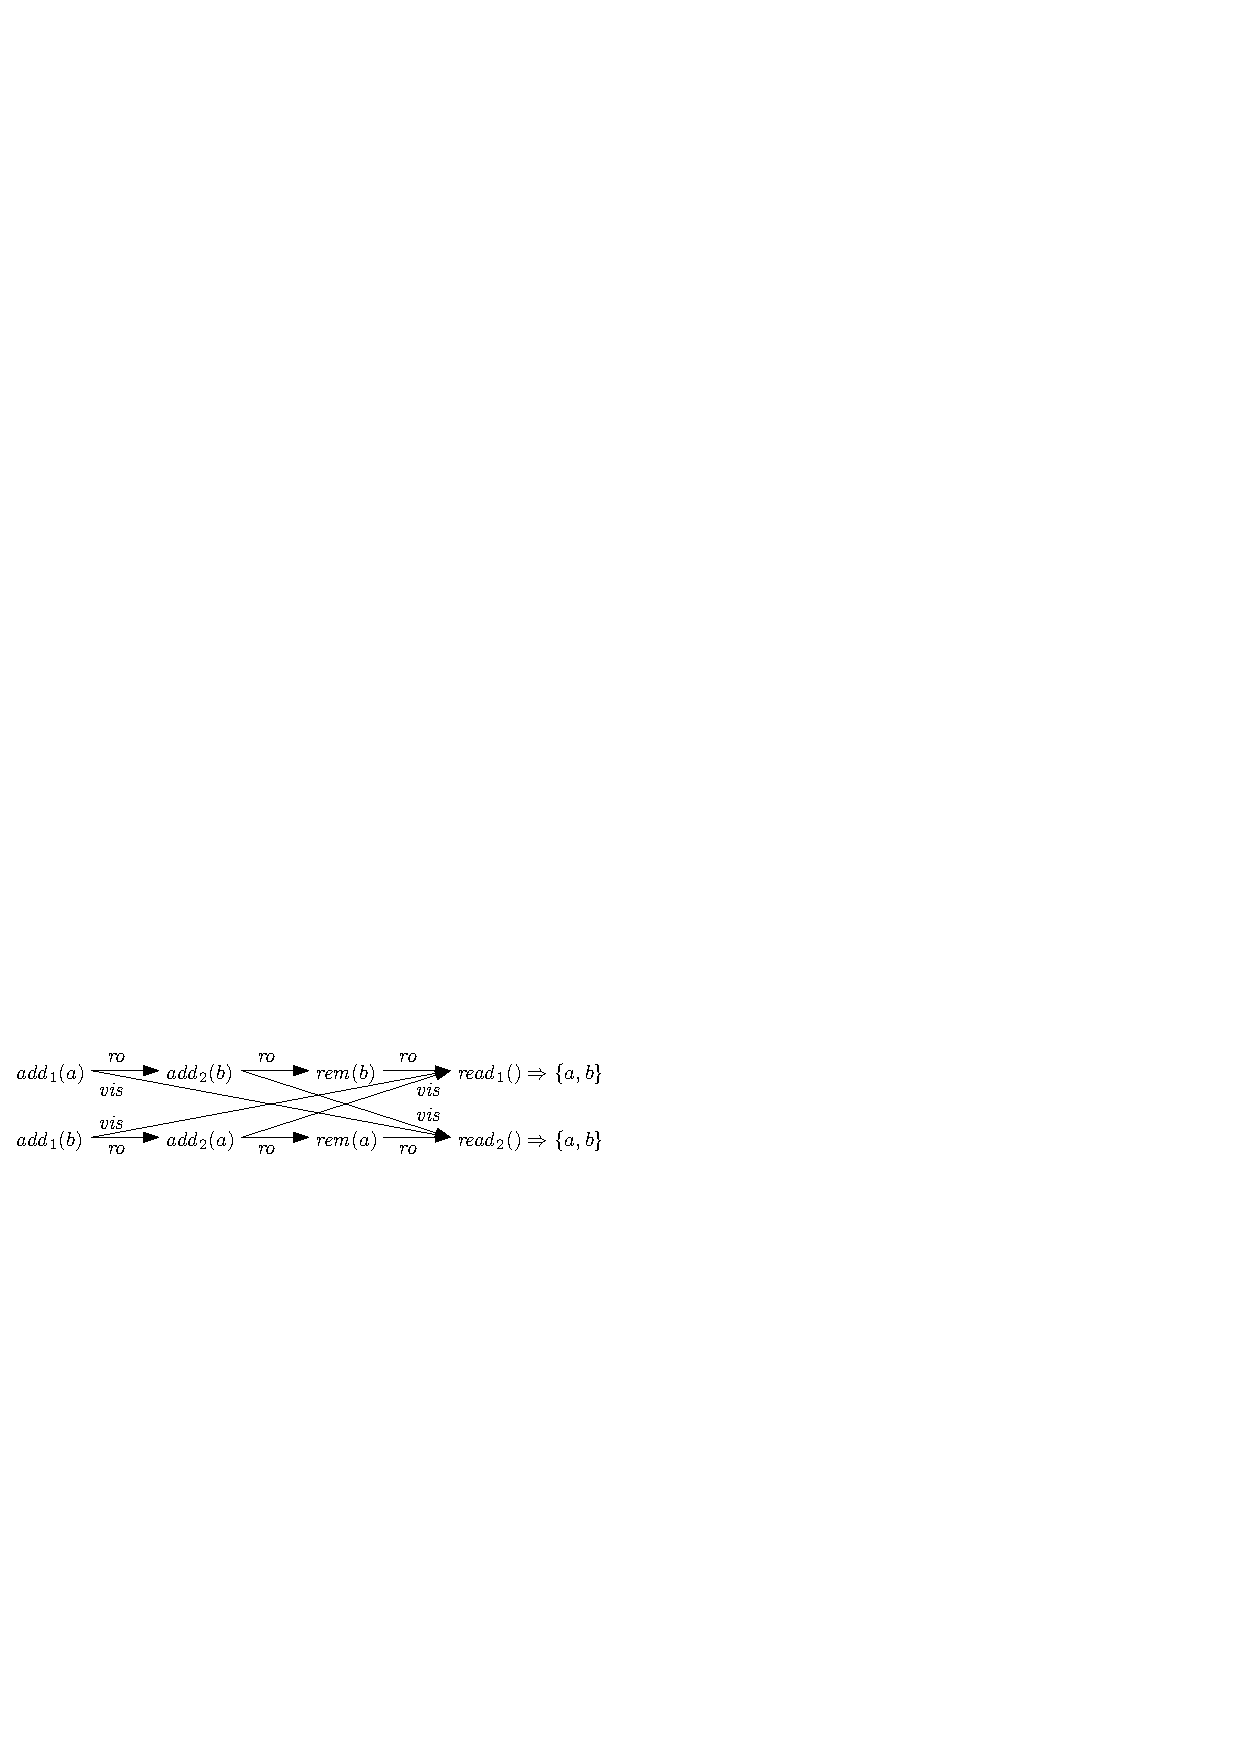
\includegraphics[width=0.7 \textwidth]{figures/PIC-His-Lin-ORSet.pdf}
%\vspace{-10pt}
%  \caption{A distributed linearizable history.}
%  \label{fig:a distributed linearizable history}
%\end{figure}

%\figurename~\ref{fig:a non-distributed linearizable history} is a history of list with add-after interface. It is not distributed linearizable w.r.t $\mathit{list}_s^{\mathit{af}}$, since the operation $\mathit{read} \Rightarrow a \cdot b \cdot c$ can not be validated. By enumerating all possible linearizations, the only possible valid return value of this $\mathit{read}$ operation are $a \cdot c \cdot b$ and $b \cdot a \cdot c$.

%\begin{figure}[t]
%  \centering
%  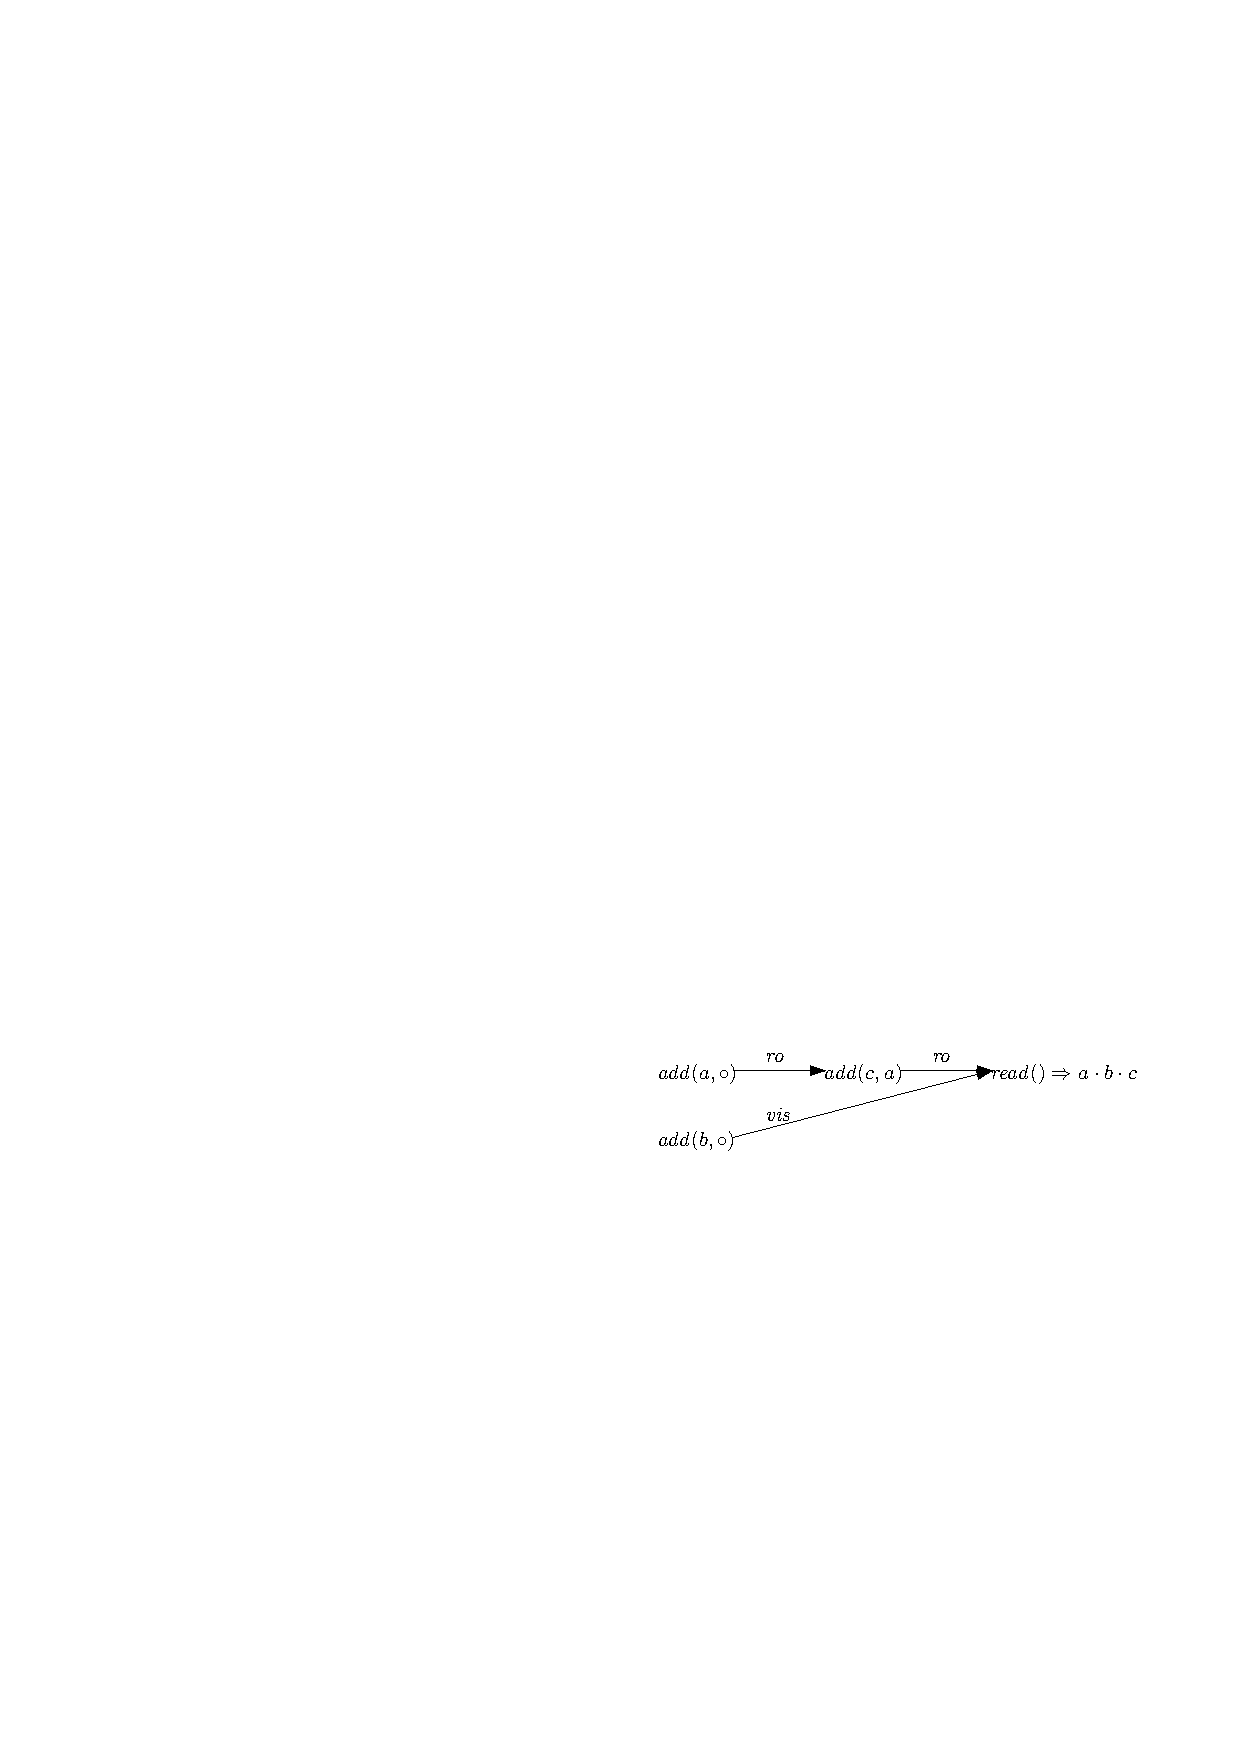
\includegraphics[width=0.6 \textwidth]{figures/PIC-Example-NonLinHis.pdf}
%\vspace{-10pt}
%  \caption{A non-distributed linearizable history.}
%  \label{fig:a non-distributed linearizable history}
%\end{figure}

We say a history satisfy convergence, if given query operations $o_1$ and $o_2$ of this history, if $o_1$ and $o_2$ see the same set of update operations, then they observe from ``a same abstract state''. Or we can say, when such $o_1$ and $o_2$ are of same method, they should return same value. A sequential specification is deterministic, if from one state and one transition label, there is at most one destination state. It is obvious that all sequential specification examples are deterministic. By definition \ref{definition:distributed linearizability}, our distributed linearizability for deterministic sequential specification obviously implies convergence, %However, this does not holds when we consider nondeterministic sequential specification. One example is shown in \figurename~\ref{fig:a non-convergent history}. It is easy to see that this history is distributed linearizable w.r.t $\mathit{list}_s^{\mathit{ab}}$. Two $\mathit{read}$ operations both see $\mathit{add}(a,\circ_1,\circ_2)$ and $\mathit{add}(b,\circ_1,\circ_2)$. However, one of them decide to put $a$ before $b$, and the other decide to put $b$ before $a$, and this implies non-convergence. 
as stated by the following lemma. 


%\begin{figure}[t]
%  \centering
%  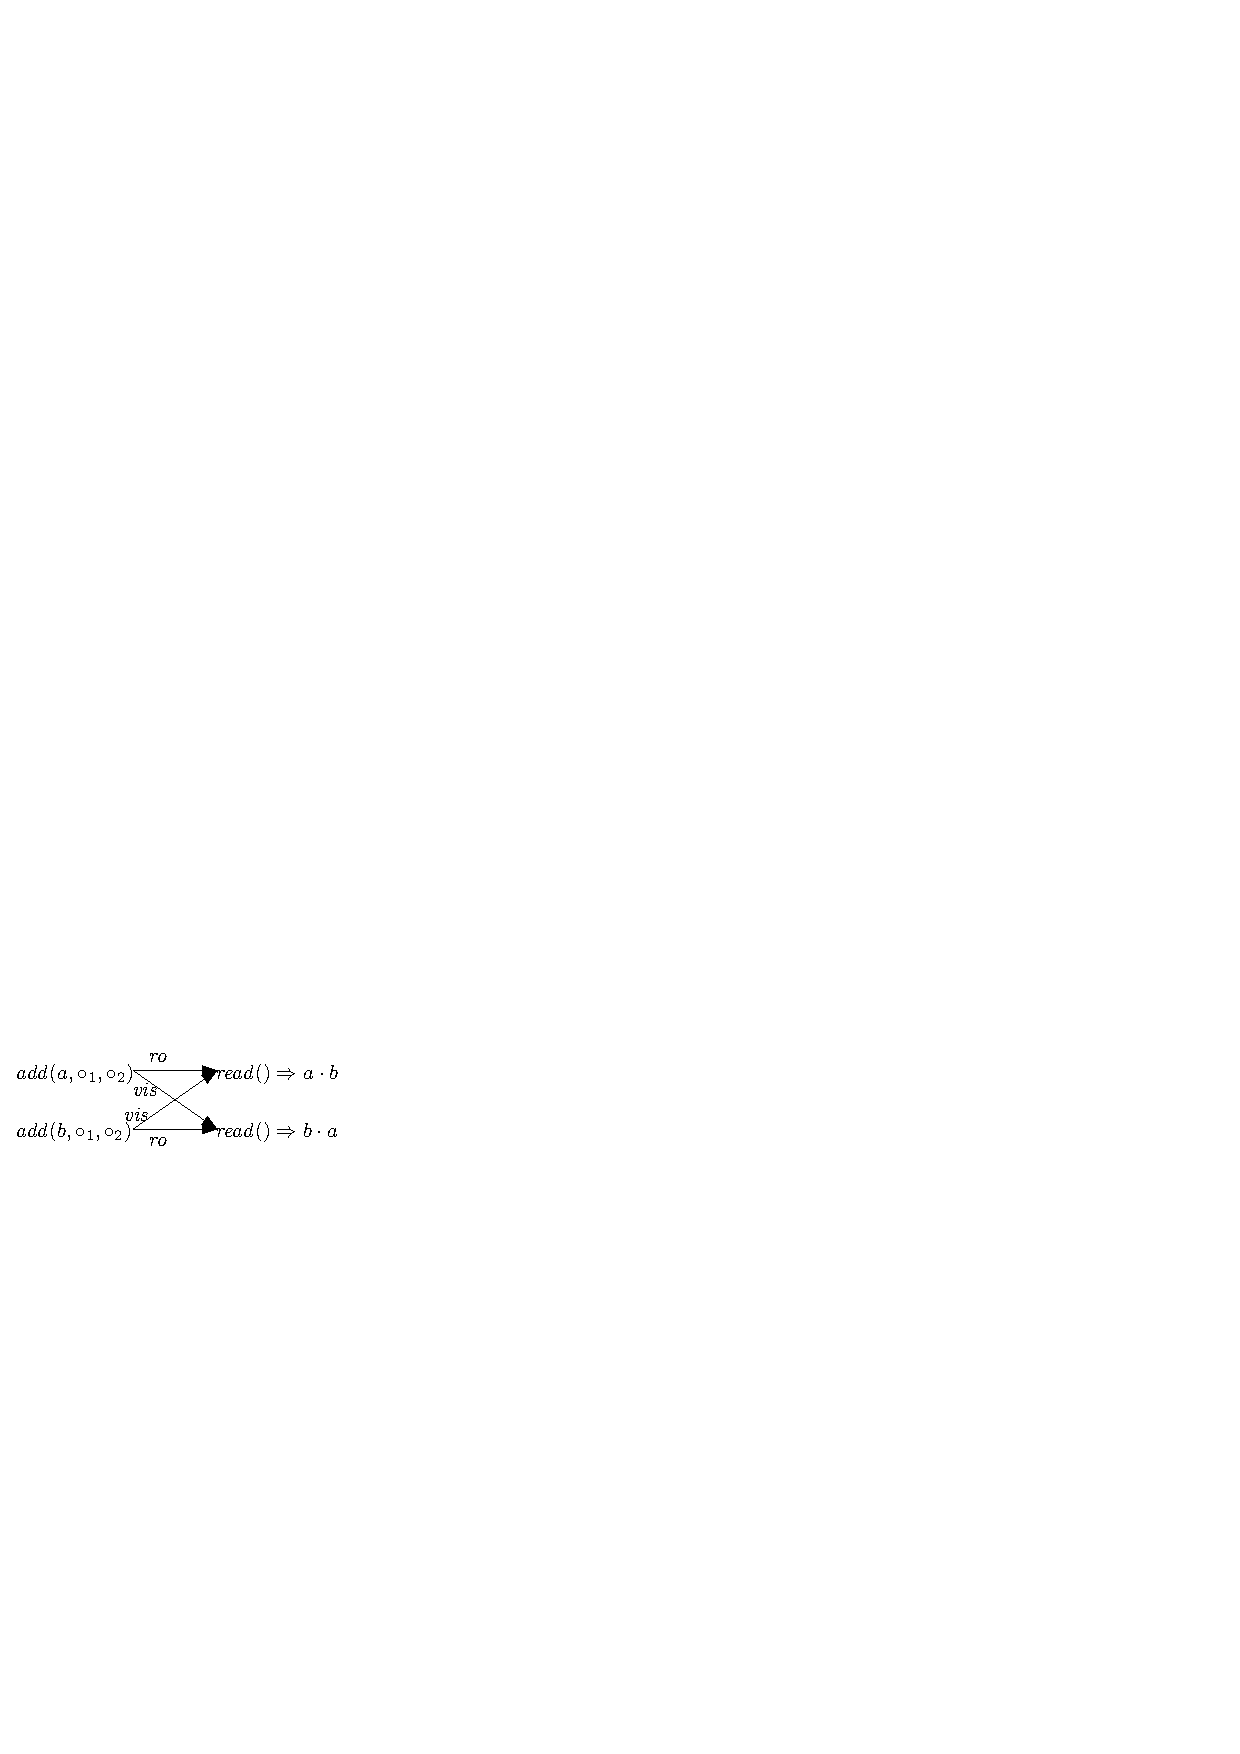
\includegraphics[width=0.4 \textwidth]{figures/PIC-His-list-NonConvergent.pdf}
%\vspace{-10pt}
%  \caption{A non-convergent history.}
%  \label{fig:a non-convergent history}
%\end{figure}



%Intuitively, we intends to use linearization to do conflict resolution. This works well for deterministic sequential specification. However, when the sequential specification becomes nondeterministic, linearization is not enough to do conflict resolution. This is the reason for this anomaly. Note that a nondeterministic sequential specification, such as $\mathit{list}_s^{\mathit{ab}}$, does not mean that in algorithm they choose random position for an item or they do conflict resolution in a random style. For example, in latter section we will see that a list algorithm called WOOT is distributed linearizable w.r.t $\mathit{list}_s^{\mathit{ab}}$, while WOOT ensures convergence. The reason for using $\mathit{list}_s^{\mathit{ab}}$ for WOOT is that: in $\mathit{add}(b,a,c)$ method of WOOT, the position of item $b$ is determined by some associated detailed information of item $b$ which is too detail for specification; and the position of $b$ is neither the immediate position after that of $a$, or the position immediate before that of $c$.

%To deal with nondeterministic sequential specification, we added an additionally condition in distributed linearization definition: Let $s_0$ be the initial state of sequential specification,

%\begin{enumerate}[(i)]
%\item For each query operation $o$, if $s_0 {\xrightarrow{ \mathit{lin} \uparrow_{ \mathit{vis}^{-1}(o)  } \cdot o }} s$, and $s_0 {\xrightarrow{ \mathit{lin} \uparrow_{ \mathbb{U} } } } s'$, then $s$ is a ``sub-state'' of $s'$.
%\end{enumerate}

%For $\mathit{list}_s^{\mathit{ab}}$ we interpret this condition as: If $s = (a_1,f_1) \cdot \ldots \cdot (a_k,b_k)$ and $s' = (a'_1,f'_1) \cdot \ldots \cdot (a'_n,f'_n)$, then $a_1 \cdot \ldots \cdot a_k$ is a sub-sequence of $a'_1 \cdot \ldots \cdot a'_n$. The following lemma states that our distributed linearizability implies convergence. It holds for $\mathit{list}_s^{\mathit{ab}}$, since our additional condition ensure that if two $\mathit{read}$ operation sees same set of $\mathit{add}$ and $\mathit{rem}$ operations, then their local state must be the same.

\begin{lemma}
\label{lemma:distributed linarizability implies convergence}
If a history $h$ is distributed linearizability w.r.t deterministic sequential specification, then $h$ satisfies convergence. 
\end{lemma}







\forget{
\section{Distributed Linearizability}
\label{sec:distributed-lin}

In this section, we propose a framework to specify the expected outcome in a linearizable approach, without referring to implementation details.



\subsection{Histories}
\label{subsec:histories}

We define our specification on histories, which are abstract version of detailed executions and does not contain implementation details such as message delivery. Histories are used to capture the notion of client-observable effects (operations), as well as their order in each replica, and their visibility relation.

Let us introduce the notion of operations. A operation label $m(a) \Rightarrow b$ with $m \in \mathbb{M}$ and $a,b \in \mathbb{D}$ is the user-observable behavior of an operation, which indicates that this operation calls method $m$ with argument $a$ and its return value is $b$. An operation is defined to be a tuple $(\ell,i,x)$, where $\ell$ is a operation label, $i \in \mathbb{OID}$ is a unique operation identifier, and $x \in \mathbb{OBJ}$ is the objects of this operation. Let $\mathbb{OP}$ be the set of operations. For operation label $m(a) \Rightarrow b$, when the argument (resp., return value) is not used, we write $m()\Rightarrow b$ (resp., $m(a)$) instead for short.

With the notion of operations, we can now define histories.

\begin{definition}[histories]
\label{definition:histories}
A history is a tuple of the form $(\mathit{Op},\mathit{ro},\mathit{vis})$ .Here $\mathit{Op} \subseteq \mathbb{OP}$ is a set of operations; $\mathit{ro} \subseteq \mathit{Op} \times \mathit{Op}$ is the replica order, which is a union of transitive, irreflexive and total orders over $\mathit{Op}$; $\mathit{vis} \subseteq \mathit{Op} \times \mathit{Op}$ is the visibility order, which is acyclic and relates operations of same object. We require that $\mathit{ro} \subseteq \mathit{vis}$.
\end{definition}

$(o_1,o_2) \in \mathit{ro}$ represents that $o_1$ and $o_2$ are of same replica and the time point of $o_1$ is before that of $o_2$. $(o_1,o_2) \in \mathit{vis}$ means that $o_2$ is aware of $o_1$. In detailed execution, this means that some message carrying the effect of $o_1$ has already been delivered into replica of $o_2$. In state-based CRDT implementation, this message contains some state aware of $o_1$, while in operation-based CRDT implementation, this message is the message of $o_1$. Based on this intuition, when $(o_1,o_2) \in \mathit{vis}$, we assume that $o_1 \in \mathbb{U}$, since otherwise $o_1 \in \mathbb{Q}$ and has no side-effect.

\subsection{Sequential Specification}
\label{subsec:sequential specification}

A sequential specification intends to propose a linearizable explanation for distributed objects.

For objects of simple types, a sequential specification is a set of operation sequences. Normally, the sequential specification is defined by the pre-condition and post-conditions. For example, the following is the sequential specification for distributed counter, and is given as a set of transition rules between states. Each state contains a integer value. Transition rule $\{ \mathit{state} = i \}$ $(\mathit{inc},\_,\_)$ $\{ \mathit{state} = i+1 \}$ indicates that $\mathit{inc}$ will increase the state by $1$. Here we use $\_$ to indicate an element whose value has no influence. Since this rule does not use operation identifier and object, it is safe to write $\{ \mathit{state} = i \}$ $\mathit{inc}$ $\{ \mathit{state} = i+1 \}$ instead. Similarly for $\mathit{dec}$ and $\mathit{read}$ operations. We write $s {\xrightarrow{o}} s'$ to indicate one step of $o$ transition between states $s$ and $s'$ that satisfies some transition rule.

A sequence $(\ell_1,i_1,x) \cdot \ldots \cdot (\ell_k,i_k,x)$ is in sequential specification $\mathit{counter}_s$, if there exists state $s_k$, such that $s_0 {\xrightarrow{(\ell_1,i_1,x)}} \ldots {\xrightarrow{(\ell_k,i_k,x)}} s_k$, and $s_0$ is the initial state. For example, it is easy to see that $(\mathit{inc},\mathit{id}_1,x) \cdot (\mathit{inc},\mathit{id}_2,x) \cdot (\mathit{dec},\mathit{id}_3,x) \cdot (\mathit{read} \Rightarrow 1,\mathit{id}_4,x) \in \mathit{counter}_s$. Note that operations of one sequence of $\mathit{counter}_s$ must be of a same object. We also implicitly assume that each operation has a unique operation identifier.


\begin{example}[sequential specification of counter]
\label{definition:sequential specification of counter}
The sequential specification $\mathit{counter}_s$ of counter is given as follows: Let $\mathit{state}$ be a integer with initial value $0$.

\begin{itemize}
\setlength{\itemsep}{0.5pt}
\item[-] $\{ \mathit{state} = i \}$ $\mathit{inc}$ $\{ \mathit{state} = i+1 \}$.
\item[-] $\{ \mathit{state} = i \}$ $\mathit{dec}$ $\{ \mathit{state} = i-1 \}$.
\item[-] $\{ \mathit{state} = i \}$ $(\mathit{read}() \Rightarrow i)$ $\{ \mathit{state} = i \}$.
\end{itemize}
\end{example}

However, for objects of some types which are designed only for distributed system, such as multi-value register and OR-set, sequential specification in above style seems insufficient (we explain this in the next subsection). To solve this problem, in the transition rules of sequential specification, for some operations, we give them a additional argument which is a set of operation identifiers. Such additional argument essentially represents the operations visible to this operation. We use the sequential specification of multi-value register as example to explain this, which is shown below.

Each state contains a set of tuples $(a,\mathit{id},f)$, where $a$ is item, $\mathit{id}$ is the operation identifier of the operation that put this tuple, and $f$ indicates whether this item is logically removed or not. Given a state $S$, a $(write(a),\mathit{id},x)$ operation with argument $S_1$, the resulting state is obtained by marking all items in $S$ with $S_1$ identifiers into $\mathit{false}$, and then insert $(a,id,\mathit{true})$ into $S$. A $\mathit{read}$ operation returns value with flag $\mathit{true}$ in state.


\begin{example}[sequential specification of multi-value register]
\label{definition:sequential specification of multi-value register}
The sequential specification $\mathit{MVReg}_s$ of multi-value register is given as follows: Let $\mathit{state}$ be a set and each its element $(a,\mathit{id},f)$ is a tuple of a data $a$, a operation identifier $\mathit{id} \in \mathbb{O}$, and a flag $f \in \{ \mathit{true},\mathit{false} \}$.
\begin{itemize}
\setlength{\itemsep}{0.5pt}
\item[-] $\{ \mathit{state} = S \}$ $((write(a),\mathit{id},x),S_1)$ $\{ \mathit{state} = S[(b,\mathit{id}_1) \in S_2 : \mathit{false}]
\cup
\{ (a,id,\mathit{true}) \}
\}$. Here $S_2 = \{ (b,\mathit{id}_1) \vert (b,\mathit{id}_1,\mathit{true}) \in S \wedge id \in S_1 \}$.
\item[-] $\{ \mathit{state} = S \wedge S_1 = \{ a \vert (a,\_,\mathit{true}) \in S \} \}$ $read() \Rightarrow S_1$ $\{ \mathit{state} = S \}$.
\end{itemize}
\end{example}

Based on above intuition, let us introduce the notion of sequential specification. Let specification alphabet $\mathbb{A} = \mathbb{OP} \cup \{ (o,s) \vert o \in \mathbb{OP}, s \subseteq \mathbb{OID} \}$. Then, a sequential specification of CRDT is defined as a set of sequences over specification alphabets $\mathbb{A}$.

%\gp{We should add the specifications (even non-deterministic here.)}
\begin{definition}[Sequential Specification]
\label{definition:sequential specification}
A sequential specification is a set of strings over specification alphabet $\mathbb{A}$.
\end{definition}

The methods that needs additional arguments, such as $\mathit{write}$ method of multi-value register and $\mathit{rem}$ method of OR-set, is called special methods of that specification. Given a sequential specification  A sequential specification is $\mathit{deterministic}$, if in each of its rules, from each state with each operation, there is at most one resulting state. Otherwise, it is a $\mathit{nondeterministic}$ specification. In the following we will introduce several types and their sequential specifications. $\mathit{list}_s^{\mathit{ab}}$, a version of list specification, is nondeterministic, while all other sequential specifications are deterministic.


\begin{example}[set and its sequential specification]
\label{definition:sequential specification of set}
A set has three methods: $\mathit{add}(a)$ inserts item $a$ into set; $\mathit{rem}(a)$ removes $a$ from set; and $\mathit{read}$ returns the set content. It implicitly assumes that each item being put into the set only once. The sequential specification $\mathit{set}_s$ of set is given as follows:  Let $\mathit{state}$ be a set and each its element $(a,f)$ is a tuple of a data $a$ and a flag $f \in \{ \mathit{true},\mathit{false} \}$.

\begin{itemize}
\setlength{\itemsep}{0.5pt}
\item[-] $\{ \mathit{state} = S \wedge a \notin S \}$ $\mathit{add}(a)$ $\{ \mathit{state} = S \cup \{ (a,\mathit{true}) \} \}$.
\item[-] $\{ \mathit{state} = S \wedge (a,\_) \in S \}$ $\mathit{rem}(a)$ $\{ \mathit{state} = S[a:\mathit{false}] \}$.
\item[-] $\{ \mathit{state} = S \wedge S_1 = \{a \vert (a,\mathit{true}) \in S \} \}$ $(\mathit{read}() \Rightarrow S_1)$ $\{ \mathit{state} = S \}$.
\end{itemize}
\end{example}



\begin{example}[OR-set and its sequential specification]
\label{definition:sequential specification of or-set}
OR-set is essential a multi-set: $\mathit{add}(a)$ inserts an item $a$ into multi-set; $\mathit{rem}(a)$ cancels only items $a$ that are inserted by $\mathit{add}(a)$ operations visible to this remove operation; $\mathit{read}$ returns the set of items in multi-set. A value can be inserted multiple times.

The sequential specification $\mathit{OR}$-$\mathit{set}_s$ of OR-set is given as follows: Let $\mathit{state}$ be a set and each its element $(a,\mathit{id},f)$ is a tuple of a data $a$, a operation identifier $\mathit{id} \in \mathbb{O}$, and a flag $f \in \{ \mathit{true},\mathit{false} \}$. In $((rem(a),\mathit{id}'),S_1)$, $S_1$ represents the operations visible to this remove operation.
\begin{itemize}
\setlength{\itemsep}{0.5pt}
\item[-] $\{ \mathit{state} = S  \wedge (\_,\mathit{id},\_) \notin S \}$ $(\mathit{add}(a),\mathit{id})$ $\{ \mathit{state} = S \cup \{ (a,\mathit{id},\mathit{true}) \} \}$.
\item[-] $\{ \mathit{state} = S \wedge S_1 = \{ a \vert (a,\_,\mathit{true}) \in S \} \}$ $(\mathit{read}() \Rightarrow S_1)$ $\{ \mathit{state} = S \}$.
\item[-] $\{ \mathit{state} = S \}$ $((rem(a),\_,\_),S_1)$ $\{ \mathit{state} = S[(b,\mathit{id}_1) \in S_2 : \mathit{false}] \}$. Here $S_2 = \{ (b,\mathit{id}_1) \vert (b,\mathit{id}_1,\mathit{true}) \in S \wedge id \in S_1 \}$.
\end{itemize}
\end{example}


\begin{example}[register and its sequential specification]
\label{definition:sequential specification of register}
A register has two methods: $\mathit{write}(a)$ writes $a$ into register; $\mathit{read}$ returns the value of register. The sequential specification $\mathit{reg}_s$ of register is given as follows: Let $\mathit{state} \in \mathbb{D}$ be a value.
\begin{itemize}
\setlength{\itemsep}{0.5pt}
\item[-] $\{ \mathit{state} = a  \}$ $\mathit{write}(b)$ $\{ \mathit{state} = b \}$.
\item[-] $\{ \mathit{state} = a \}$ $(\mathit{read}() \Rightarrow a)$ $\{ \mathit{state} = a \}$.
\end{itemize}
\end{example}




\begin{example}[List with add-after interface]
\label{definition:sequential specification of list with add-after interface}
Assume each item of the list is unique. A list has three methods: $\mathit{add}(b,a)$ inserts item $b$ into the list at the position immediately after that of item $a$; $\mathit{rem}(a)$ removes item $a$ from the list; and $\mathit{read}$ returns the list content. We assume that the initial value of list is $(\circ,\mathit{true})$ and this node can not be removed. We use the word ``add-after'' to emphasize the method $\mathit{add}(b,a)$, which is different from the other list interface that uses method $\mathit{add}(b,a,c)$.

The sequential specification $\mathit{list}_s^{\mathit{af}}$ of list is given as follows: Let $\mathit{state}$ be a sequence, where each item is a tuple $(a,f)$ with data $a$ and flag $f \in \{ \mathit{true},\mathit{false} \}$. Here $\mathit{af}$ represents add-after, and we use $l \uparrow_{S}$ to represent the projection of sequence $l$ into set $S$. When the context is clear, in $\mathit{read}$ operation, we will omit $\circ$.
\begin{itemize}
\setlength{\itemsep}{0.5pt}
\item[-] $\{ \mathit{state} = (a_1,f_1) \cdot \ldots \cdot (a_n,f_n) \wedge l \leq n \wedge b \notin \{ a_1, \ldots, a_n \} \}$ $add(b,a_l)$ $\{ \mathit{state} = (a_1,f_1) \cdot \ldots \cdot (a_l,f_l) \cdot (b,\mathit{true}) \cdot (a_{l+1},f_{l+1}) \cdot \ldots \cdot (a_n,f_n) \}$.
\item[-] $\{ \mathit{state} = (a_1,f_1) \cdot \ldots \cdot (a_n,f_n) \wedge S = \{ a \vert (a,\mathit{true}) \in \mathit{state} \} \wedge l = a_1 \cdot \ldots \cdot a_n \uparrow_{S} \}$ $(read() \Rightarrow l)$ $\{ \mathit{state} = (a_1,f_1) \cdot \ldots \cdot (a_n,f_n) \}$.
\end{itemize}
\end{example}



\begin{example}[List with add-between interface]
\label{definition:sequential specification of list with add-after interface}
Such kind of list is similar as list with add-after interface. One difference is the $\mathit{add}$ method: $\mathit{add}(b,a,c)$ inserts item $b$ into the list at some nondeterministic position between position of $a$ and position of $c$. The other difference is that, we assume that the initial value of list is $(\circ_1,\mathit{true}) \cdot (\circ_2,\mathit{true})$ and these two nodes can not be removed. The sequential specification $\mathit{list}_s^{\mathit{ab}}$ of list is given as follows: Here $\mathit{ab}$ represents add-between. When the context is clear, in $\mathit{read}$ operation, we will omit $\circ_1$ and $\circ_2$.
\begin{itemize}
\setlength{\itemsep}{0.5pt}
\item[-] $\{ \mathit{state} = (a_1,f_1) \cdot \ldots \cdot (a_n,f_n) \wedge k < m < l \wedge b \notin \{ a_1, \ldots, a_n \} \}$ $add(b,a_k,a_l)$ $\{ \mathit{state} = (a_1,f_1) \cdot \ldots \cdot (a_m,f_m) \cdot (b,\mathit{true}) \cdot (a_{m+1},f_{m+1}) \cdot \ldots \cdot (a_n,f_n) \}$. Here the chosen of $m$ is deterministic.
\item[-] $\{ \mathit{state} = (a_1,f_1) \cdot \ldots \cdot (a_n,f_n) \wedge S = \{ a \vert (a,\mathit{true}) \in \mathit{state} \} \wedge l = a_1 \cdot \ldots \cdot a_n \uparrow_{S} \}$ $(read() \Rightarrow l)$ $\{ \mathit{state} = (a_1,f_1) \cdot \ldots \cdot (a_n,f_n) \}$.
\end{itemize}
\end{example}







\subsection{Definition of Distributed Linearizability}
\label{subsec:definition of distributed linearizability}

A history is single-object, if it contains operations of a single object. A history is multi-object, if it contains operations of multiple objects. In the following we propose distributed linearizability for histories.


\begin{definition}[Distributed Linearizability]
\label{definition:distributed linearizability}

A single-object history $h = (\mathit{Op},\mathit{ro},\mathit{vis})$ is distributed linearizable w.r.t a deterministic sequential specification $\mathit{spec}$, if there exists a sequence $\mathit{lin}$, called linearization of $h$, such that

\begin{enumerate}[(i)]
\item The elements of $\mathit{lin}$ is generated from the operations of $h$: for operation $o$ of special methods, $\mathit{lin}$ uses $(o,\mathit{vis}^{-1}(o))$; while for other operation $o$, $\mathit{lin}$ uses $o$.
\item $\mathit{lin}$ is consistent with $\mathit{vis}$,
\item the projection of $\mathit{lin}$ into update operations is in $\mathit{spec}$,
\item For each query operation $o$, $\mathit{lin} \uparrow_{ \mathit{vis}^{-1}(o)  } \cdot o \in \mathit{spec}$.
\end{enumerate}

A multi-object history $h$ is distributed linearizable w.r.t deterministic sequential specifications, if for each object $x$, $h \uparrow_{x}$ is distributed linearizable w.r.t its sequential specification. A set $H$ of histories are distributed linearizable w.r.t deterministic sequential specifications, if each of its history is.
\end{definition}

$h \uparrow_{x}$ is obtained from $h$ by projecting the operations and relations into operations of object $x$. Here the linearization gives a global and linearizable explanation of all operations. With sequential specification and linearization of the history, the understanding of distributed behaviors should be simplified. The linearization can be also considered as a guide to the conflict resolution.

\figurename~\ref{fig:a distributed linearizable history} is a history of OR-set. Here subscript of $\mathit{add}_1(a)$ is used to distinguish different $\mathit{add}(a)$ operations, and similarly for $\mathit{read}_1() \Rightarrow \{ a,b \}$. This history is distributed linearizable. To explain this, let the operation identifiers of operations of the first replica (resp., of the second replica) be $\mathit{id}_1,\mathit{id}_2,\mathit{id}_3,\mathit{id}_4$ (resp., $\mathit{id}_5,\mathit{id}_6,\mathit{id}_7,\mathit{id}_8$), in the replica order, respectively. The linearization of this history is $\mathit{add}_1(a) \cdot \mathit{add}_1(b) \cdot \mathit{add}_2(b) \cdot \mathit{add}_2(a) \cdot ((\mathit{rem}(b),\_,\_),\{ \mathit{id}_1, \mathit{id}_2 \}) \cdot ((\mathit{rem}(a),\_,\_),\{ \mathit{id}_5, \mathit{id}_6 \}) \cdot ((\mathit{read}_1 \Rightarrow \{ a,b \},\_,\_), S ) \cdot ((\mathit{read}_2 \Rightarrow \{ a,b \},\_,\_), S )$, where $S = \{ \mathit{id}_1, \mathit{id}_2, \mathit{id}_3, \mathit{id}_5, \mathit{id}_6, \mathit{id}_7 \}$.

The history of \figurename~\ref{fig:a distributed linearizable history} is distributed linearizable w.r.t $\mathit{OR}$-$\mathit{set}_s$, but not $\mathit{set}_s$. Assume that by contradiction, this history is linearizable w.r.t $\mathit{set}_s$ and $\mathit{lin}$ is its linearization. Then it is obvious that to ensure $b$ be in the return value of $\mathit{read}_1$, we should put $\mathit{add}_1(b)$ after $\mathit{rem}(b)$ in $\mathit{lin}$; then $\mathit{add}_2(a)$ is after $\mathit{add}_1(b)$ in in $\mathit{lin}$, and $\mathit{rem}(a)$ is after $\mathit{add}_2(a)$ in in $\mathit{lin}$. However, this makes $a$ not in return value of $\mathit{read}_2$ according to $\mathit{set}_s$, which introduces contradiction. Therefore, it seems quite difficult to have a sequential specification of OR-set without using special methods.

\begin{figure}[t]
  \centering
  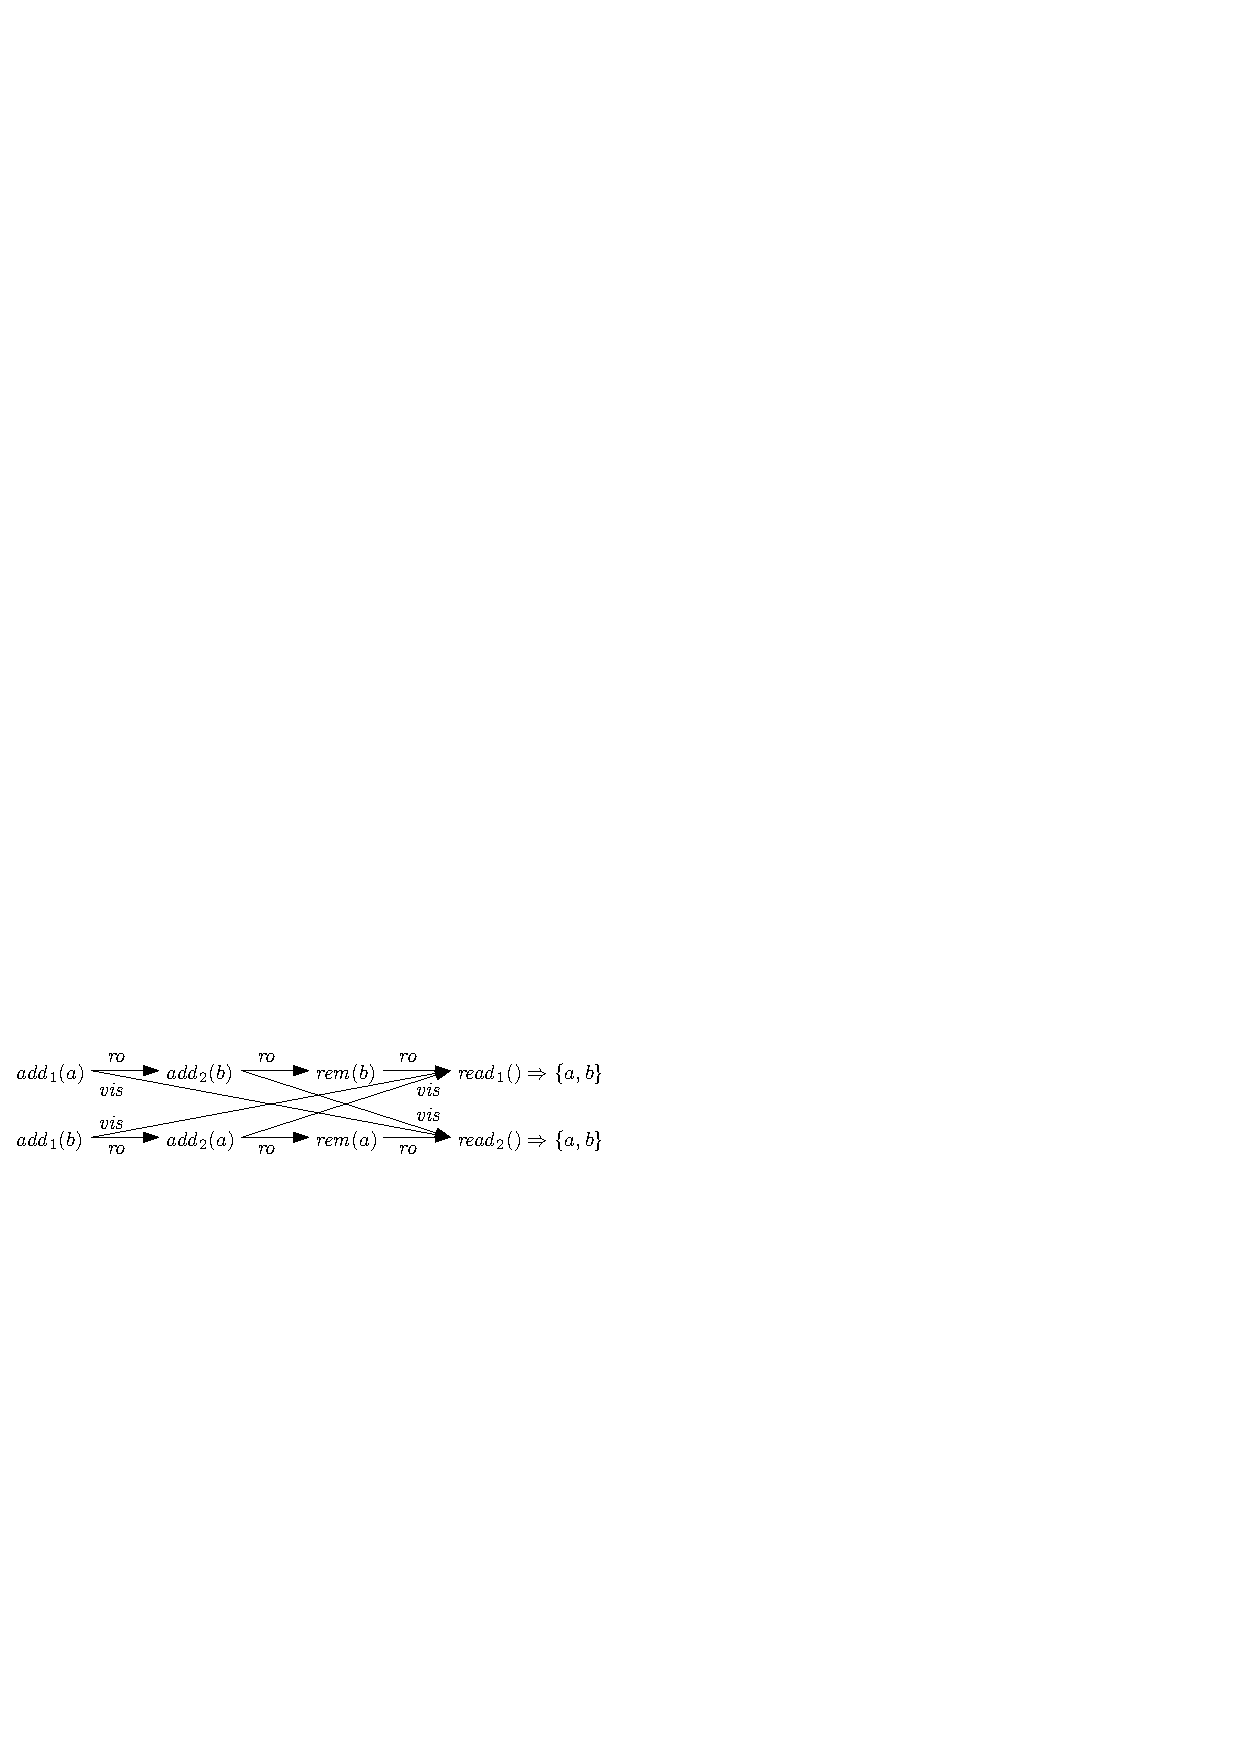
\includegraphics[width=0.7 \textwidth]{figures/PIC-His-Lin-ORSet.pdf}
%\vspace{-10pt}
  \caption{A distributed linearizable history.}
  \label{fig:a distributed linearizable history}
\end{figure}

\figurename~\ref{fig:a non-distributed linearizable history} is a history of list with add-after interface. It is not distributed linearizable w.r.t $\mathit{list}_s^{\mathit{af}}$, since the operation $\mathit{read} \Rightarrow a \cdot b \cdot c$ can not be validated. By enumerating all possible linearizations, the only possible valid return value of this $\mathit{read}$ operation are $a \cdot c \cdot b$ and $b \cdot a \cdot c$.

\begin{figure}[t]
  \centering
  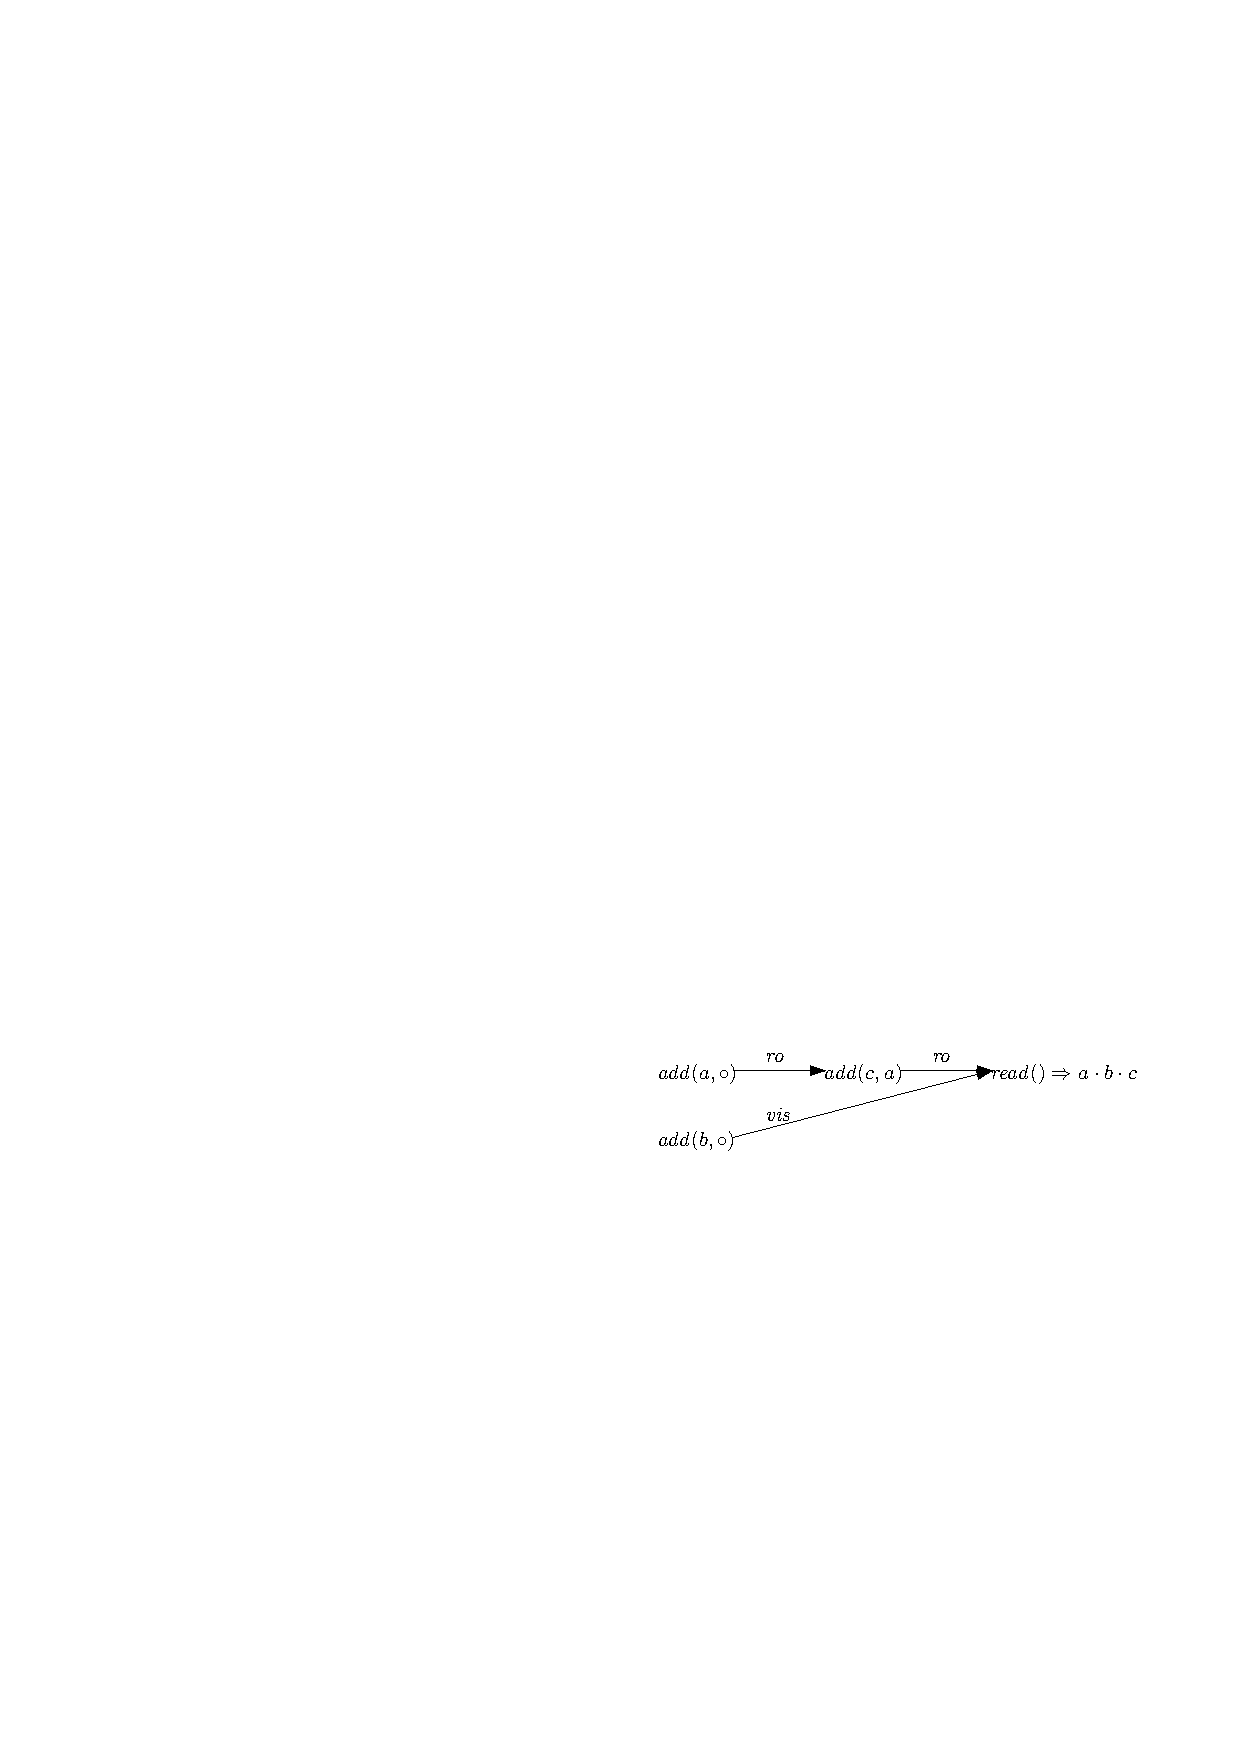
\includegraphics[width=0.6 \textwidth]{figures/PIC-Example-NonLinHis.pdf}
%\vspace{-10pt}
  \caption{A non-distributed linearizable history.}
  \label{fig:a non-distributed linearizable history}
\end{figure}

We say a history satisfy convergence, if given query operations $o_1$ and $o_2$ of this history, if $o_1$ and $o_2$ see the same set of update operations, then they observe from ``a same abstract state''. Or we can say, when such $o_1$ and $o_2$ are of same method, they should return same value. By definition \ref{definition:distributed linearizability}, our distributed linearizability for deterministic sequential specification obviously implies convergence. However, this does not holds when we consider nondeterministic sequential specification. One example is shown in \figurename~\ref{fig:a non-convergent history}. It is easy to see that this history is distributed linearizable w.r.t $\mathit{list}_s^{\mathit{ab}}$. Two $\mathit{read}$ operations both see $\mathit{add}(a,\circ_1,\circ_2)$ and $\mathit{add}(b,\circ_1,\circ_2)$. However, one of them decide to put $a$ before $b$, and the other decide to put $b$ before $a$, and this implies non-convergence.


\begin{figure}[t]
  \centering
  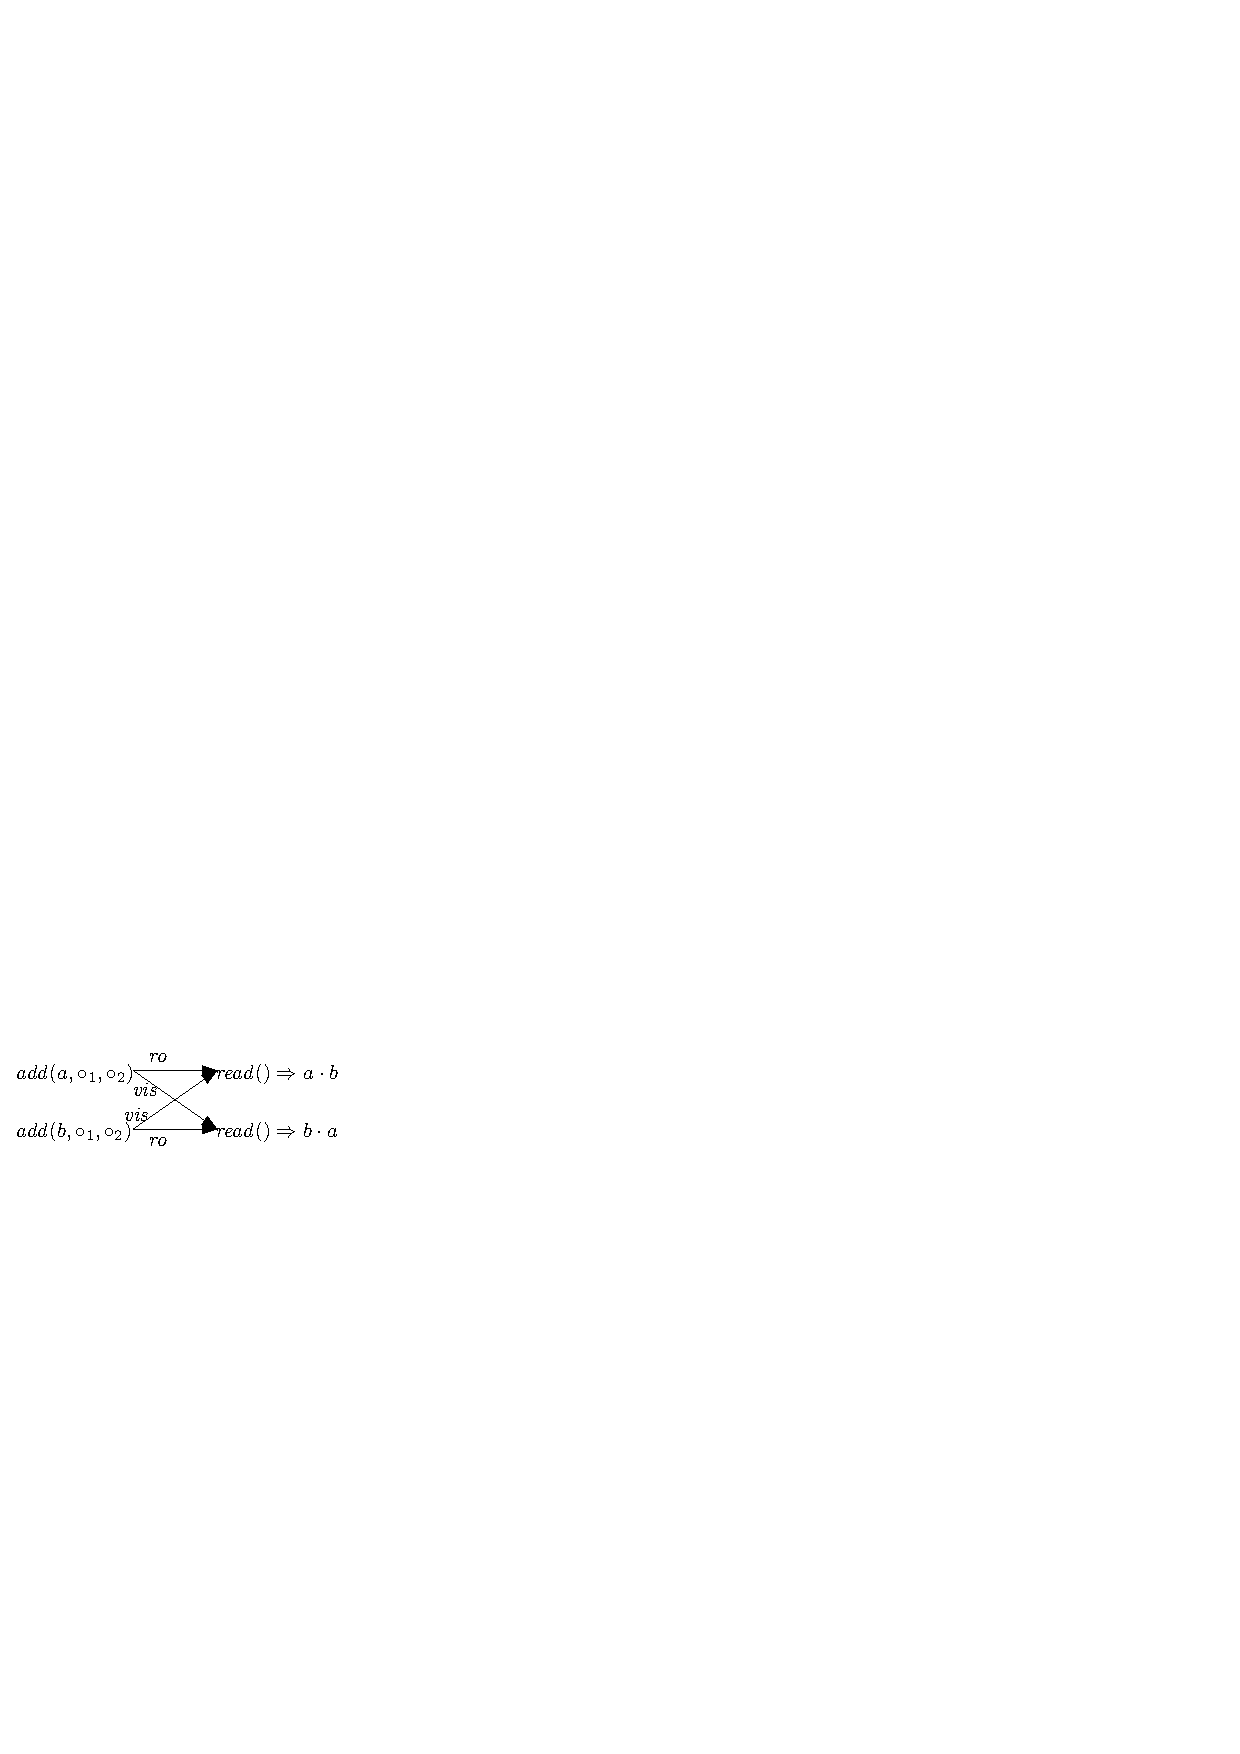
\includegraphics[width=0.4 \textwidth]{figures/PIC-His-list-NonConvergent.pdf}
%\vspace{-10pt}
  \caption{A non-convergent history.}
  \label{fig:a non-convergent history}
\end{figure}



Intuitively, we intends to use linearization to do conflict resolution. This works well for deterministic sequential specification. However, when the sequential specification becomes nondeterministic, linearization is not enough to do conflict resolution. This is the reason for this anomaly. Note that a nondeterministic sequential specification, such as $\mathit{list}_s^{\mathit{ab}}$, does not mean that in algorithm they choose random position for an item or they do conflict resolution in a random style. For example, in latter section we will see that a list algorithm called WOOT is distributed linearizable w.r.t $\mathit{list}_s^{\mathit{ab}}$, while WOOT ensures convergence. The reason for using $\mathit{list}_s^{\mathit{ab}}$ for WOOT is that: in $\mathit{add}(b,a,c)$ method of WOOT, the position of item $b$ is determined by some associated detailed information of item $b$ which is too detail for specification; and the position of $b$ is neither the immediate position after that of $a$, or the position immediate before that of $c$.

To deal with nondeterministic sequential specification, we added an additionally condition in distributed linearization definition: Let $s_0$ be the initial state of sequential specification,

\begin{enumerate}[(i)]
\item For each query operation $o$, if $s_0 {\xrightarrow{ \mathit{lin} \uparrow_{ \mathit{vis}^{-1}(o)  } \cdot o }} s$, and $s_0 {\xrightarrow{ \mathit{lin} \uparrow_{ \mathbb{U} } } } s'$, then $s$ is a ``sub-state'' of $s'$.
\end{enumerate}

For $\mathit{list}_s^{\mathit{ab}}$ we interpret this condition as: If $s = (a_1,f_1) \cdot \ldots \cdot (a_k,b_k)$ and $s' = (a'_1,f'_1) \cdot \ldots \cdot (a'_n,f'_n)$, then $a_1 \cdot \ldots \cdot a_k$ is a sub-sequence of $a'_1 \cdot \ldots \cdot a'_n$. The following lemma states that our distributed linearizability implies convergence. It holds for $\mathit{list}_s^{\mathit{ab}}$, since our additional condition ensure that if two $\mathit{read}$ operation sees same set of $\mathit{add}$ and $\mathit{rem}$ operations, then their local state must be the same.

\begin{lemma}
\label{lemma:distributed linarizability implies convergence}
If a history $h$ is distributed linearizability w.r.t deterministic sequential specification or $\mathit{list}_s^{\mathit{ab}}$, then $h$ satisfies convergence.
\end{lemma}
}

%%% Local Variables:
%%% mode: latex
%%% TeX-master: "draft"
%%% End:
